\documentclass[UTF-8, a4paper, 11pt]{article}

\usepackage{xeCJK}
\usepackage{graphicx}
\graphicspath{{figure/}}
\usepackage[unicode]{hyperref}
\hypersetup{colorlinks=true,linkcolor=black}
\usepackage{cite}
\usepackage{indentfirst}
\usepackage{amsmath}
\numberwithin{equation}{section}
\usepackage{listings}
\usepackage{xcolor}
\usepackage{fontspec}
\usepackage{courier}
\usepackage{tikz-timing}

\lstset{
    basicstyle=\scriptsize\ttfamily,
    numbers=left,                                        % 在左侧显示行号
    keywordstyle=\color[RGB]{40,40,255},                 % 设定关键字颜色
    frame=trbl,
    numberstyle=\scriptsize\color{darkgray},           % 设定行号格式
    commentstyle=\it\color[RGB]{0,96,96},                % 设置代码注释的格式
    stringstyle=\ttfamily\slshape\color[RGB]{128,0,0},   % 设置字符串格式
    showstringspaces=false,                              % 不显示字符串中的空格
    language=python,                                     % 设置语言
}


\linespread{1.0}
\setlength{\parskip}{0.5\baselineskip}

\makeatletter
\let\@afterindentfalse\@afterindenttrue
\@afterindenttrue
\makeatother
\setlength{\parindent}{2em}

\addtolength{\topmargin}{-70pt}
\setlength{\oddsidemargin}{0.63cm}
\setlength{\evensidemargin}{\oddsidemargin}
\setlength{\textwidth}{15.66cm}
\setlength{\textheight}{25.00cm}

\newcommand{\chuhao}{\fontsize{42pt}{\baselineskip}\selectfont}
\newcommand{\xiaochuhao}{\fontsize{36pt}{\baselineskip}\selectfont}
\newcommand{\yihao}{\fontsize{28pt}{\baselineskip}\selectfont}
\newcommand{\erhao}{\fontsize{21pt}{\baselineskip}\selectfont}
\newcommand{\xiaoerhao}{\fontsize{18pt}{\baselineskip}\selectfont}
\newcommand{\sanhao}{\fontsize{15.75pt}{\baselineskip}\selectfont}
\newcommand{\sihao}{\fontsize{14pt}{\baselineskip}\selectfont}
\newcommand{\xiaosihao}{\fontsize{12pt}{\baselineskip}\selectfont}
\newcommand{\wuhao}{\fontsize{10.5pt}{\baselineskip}\selectfont}
\newcommand{\xiaowuhao}{\fontsize{9pt}{\baselineskip}\selectfont}
\newcommand{\liuhao}{\fontsize{7.875pt}{\baselineskip}\selectfont}
\newcommand{\qihao}{\fontsize{5.25pt}{\baselineskip}\selectfont}

\begin{document}

\begin{titlepage}
    \begin{center}
    \phantom{Start!}
	\vspace{2cm}
	
\includegraphics[width=350pt]{HUST.pdf} \\
    \vspace{1cm}
     \center{
       	  \textbf{\yihao 实\quad 验\quad 报\quad 告}\\
       	  \vspace{0.5cm}
          \textbf{\sanhao (2017 / 2018学年\quad 第2学期)}
      }
      \vspace{2.5cm}
      \begin{table}[!hbp]
      \centering
      \renewcommand\arraystretch{1.5}
     	\begin{tabular}{|c|c|}
     		\hline
     		课程名称 & 机器学习导论 \\
     		\hline
     		实验名称 & ~~~~~~Naive Bayes Classifier~~~~~~ \\
     		\hline
     		实验时间&\multicolumn{1}{c|}{2018年5月28日}\\
     		\hline
     		指导教师 & 王邦 \\
     		\hline
     		\end{tabular}     		
       \end{table}
       \vspace{2cm}
      \begin{table}[htbp]
      \centering
      \renewcommand\arraystretch{1.5}
     	\begin{tabular}{|c|c|c|c|}
     		\hline
            \qquad ~~姓名~~~~~  & \qquad ~~游浩然~~~~~  & \qquad 学号~~~~~ & \qquad U201515429~~~~~ \\
     		\hline
     		\end{tabular}
       \end{table}
       \date{2018年5月20日}
     \end{center}
\end{titlepage}

\section{问题重述}
\begin{itemize}
  \item 基于朴素贝叶斯分类器原理,使用Python编程语言实现对垃圾邮件和正常邮件的分类,输出测试集中的邮件所属类型。
\end{itemize}

\section{Naive Bayes}
\subsection{文本分类原理}
针对不同的文本,我们可以将所有出现的字母或符合作为数据特征向量,统计每个文本中词条的数目作为数据向量。简单起见, 我们采用是否出现该词条的二元变量来构为数据向量, 本文的数据集中词条有$V=87$种。
假设邮件中的内容包含的词条为$w_i$, 垃圾邮件记作Spam, 正常邮件记作ham。根据Bayes' Theorem:
\begin{equation}\label{ep:eqs}
  P(S|W)=\frac{P(W|S) \cdot P(S)}{P(W)} = \frac{P(S)}{P(W)}\times \prod_{i=1}^{V} P(W_i|S)
\end{equation}
我们的目标是求出$P(S_j|W)$,这里的$j$有两类,一类是Spam,一类是Ham。通过比较可以判断将文本划归为哪一类。在比较过程中分母相同,不予考虑。

在实际编程中,有两个问题:
\begin{enumerate}
  \item 当词条不存在时,$P(W_i|S)=0$,会造成$P(S|W)=0$,影响比较,采用M-estimation(Sec \ref{m-estimation})来避免这种问题。
  \item 当$P(W_i|S)$过小时,连乘操作会造成下溢出问题,为此,在等式两边同取$\log$,将连乘变为连加。
\end{enumerate}

\subsection{M估计}
\label{m-estimation}
M-estimation 的基本思想是扩充数据项,通过先验概率来模拟各词条占比。因此,条件概率项变为:
\begin{equation}\label{ep:eqs}
  P(W_i|S_j) = \frac{N_{Wi,Sj}}{N_{Sj}} \Longrightarrow \frac{N_{Wi,Sj}+Mp}{N_{Sj}+M}
\end{equation}
本次实验中实现了M估计的Bernouli模型$(m=2,p=\frac{1}{2})$和Polynoimal模型$(m=|V|, p=\frac{1}{|V|})$。
\subsection{Python Code}
\subsubsection{naive bayes}
\begin{lstlisting}[language=python]
# -*- coding: utf-8 -*-
"""
@author : Haoran You

"""
import os
import csv
import numpy as np
from collections import defaultdict
import matplotlib.pyplot as plt

class naive_bayes():
    def name(self):
        return 'naive bayes classifier'

    def train(self, dataset, classes, m='bernouli'):
        """
        :param dataset: all doc_vectors
        :param classes: spam or not
        :param m : m-esitmation methods
        condition_prob : conditional probability p(w|s)
        cls_prob : prior probability p(s)
        """
        sub_dataset = defaultdict(list)
        cls_cnt = defaultdict(lambda :0)
        for doc_vector, cls in zip(dataset, classes):
            sub_dataset[cls].append(doc_vector)
            cls_cnt[cls] += 1
        self.cls_prob = {k: v/len(classes) for k, v in cls_cnt.items()}
        self.condition_prob = {}
        dataset = np.array(dataset)
        for cls, sub_dataset in sub_dataset.items():
            # m-estimation
            sub_dataset = np.array(sub_dataset)
            if m == 'bernouli':
                self.condition_prob[cls] = np.log((np.sum(sub_dataset, axis=0) + 1)
                                                / (np.sum(dataset, axis=0) + 2))
            elif m == 'polynomial':
                self.condition_prob[cls] = np.log((np.sum(sub_dataset, axis=0) + 1)
                                                / (np.sum(dataset, axis=0) + len(sub_dataset[0])))
            else:
                self.condition_prob[cls] = np.log(np.sum(sub_dataset, axis=0)
                                                / np.sum(dataset, axis=0))

    def classify(self, doc_vector):
        posterior = {}
        for cls, cls_prob in self.cls_prob.items():
            condition_prob_vec = self.condition_prob[cls]
            posterior[cls] = np.sum(condition_prob_vec * doc_vector) + np.log(cls_prob)
        return max(posterior, key=posterior.get)

    def test(self, dataset, classes):
        error = 0
        for doc_vector, cls in zip(dataset, classes):
            pred = self.classify(doc_vector)
            print('Predict: {} --- Actual: {}'.format(pred, cls))
            if pred != cls:
                error += 1
        print('Error rate: {}'.format(error/len(classes)))

    def predict(self, dataset):
        if os.path.exists('results.csv'):
            os.remove('results.csv')
        f = open('results.csv', 'a', newline='')
        csv_write = csv.writer(f, dialect='excel')
        i = 0
        for doc_vector in dataset:
            result = []
            i += 1
            pred = self.classify(doc_vector)
            result.append(i)
            result.append(pred)
            csv_write.writerow(result)

    def plot(self):
        fig = plt.figure()
        ax = fig.add_subplot(111)
        for cls, prob in self.condition_prob.items():
            ax.scatter(np.arange(0, len(prob)),
                       prob*self.cls_prob[cls],
                       label=cls,
                       alpha=0.3)
            ax.legend()
        plt.show()
        plt.savefig
\end{lstlisting}
\subsubsection{data}
\begin{lstlisting}[language=python]
# -*- coding: utf-8 -*-
"""
@author : Haoran You

"""
import os
import itertools
import random

def get_doc_vector(words, vocabulary):
    doc_vector = [0] * len(vocabulary)
    for word in words:
        if word in vocabulary:
            idx = vocabulary.index(word)
            doc_vector[idx] = 1
    return doc_vector

def parse_file(dir, vocabulary, word_vector, classes, has_cls=True):
    dir_list = os.listdir(dir)
    dir_list.sort(key=lambda x:int(x[:-4]))
    for i in range(0, len(dir_list)):
        path = os.path.join(dir, dir_list[i])
        if os.path.isfile(path):
            words = []
            with open(path, 'r', encoding='ISO-8859-1') as f:
                for line in f:
                    if line:
                        vocabulary.extend(line.strip())
                        words.append(line.strip())
                        words.append(' ')
            if has_cls: classes.append(dir[13:-1])
            word_vector.append(''.join(itertools.chain(words)))
    vocabulary = list(set(vocabulary))
    if has_cls:
        return vocabulary, word_vector, classes
    else:
        return vocabulary, word_vector

def split_val(dataset, cls):
    for i in range(0, len(dataset)):
        dataset[i].append(cls[i])
    train = random.sample(dataset, int(0.8*len(dataset)))
    val = random.sample(dataset, len(dataset)-int(0.8*len(dataset)))
    # val = [example for example in dataset if example not in train]
    train_dataset, train_cls, val_dataset, val_cls = [], [], [], []
    for i in range(0, len(train)):
        train_cls.append(train[i][-1])
        train_dataset.append(train[i][:-1])
    for i in range(0, len(val)):
        val_cls.append(val[i][-1])
        val_dataset.append(val[i][:-1])
    return train_dataset, train_cls, val_dataset, val_cls

def dataset():
    vocabulary, train_word_vector, train_cls = parse_file('./train_data/ham/', [], [], [])
    vocabulary, train_word_vector, train_cls = parse_file('./train_data/spam/',
                                                 vocabulary, train_word_vector, train_cls)
    vocabulary, test_word_vector = parse_file('./test_data/', vocabulary, [], [], False)
    train_dataset = [get_doc_vector(words, vocabulary) for words in train_word_vector]
    test_dataset = [get_doc_vector(words, vocabulary) for words in test_word_vector]
    train_dataset, train_cls, val_dataset, val_cls = split_val(train_dataset, train_cls)
    print('num of trainset : ', len(train_dataset))
    print('num of valset   : ', len(val_dataset))
    print('num of testset  : ', len(test_dataset))
    return train_dataset, train_cls, val_dataset, val_cls, test_dataset
\end{lstlisting}
\newpage
\subsubsection{Main}
\begin{lstlisting}[language=python]
# -*- coding: utf-8 -*-
"""
@author : Haoran You

"""
from nb_for_spam import naive_bayes
from data import *

# dataset
train_dataset, train_cls, val_dataset, val_cls, test_dataset = dataset()
# train
nb = naive_bayes()
nb.train(train_dataset, train_cls)
nb.plot()
# val
nb.test(val_dataset, val_cls)
# test
nb.predict(test_dataset)
\end{lstlisting}
\subsubsection{Conditional Probability Visualization}
\begin{figure}[!htbp]
  \centering
  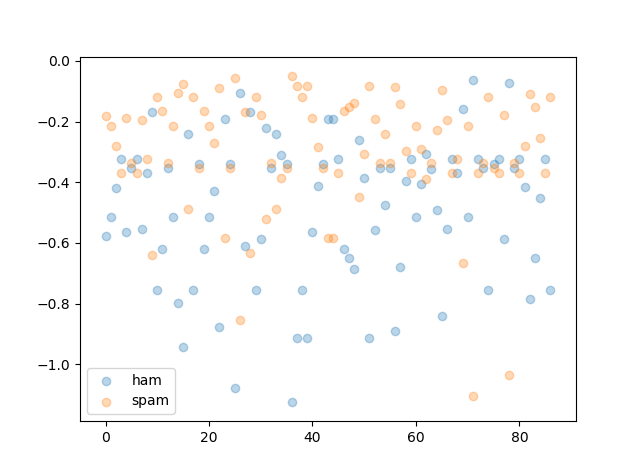
\includegraphics[width=16cm]{cond_fig.png}
  \caption{Conditional Probability Visualization}\label{condition}
\end{figure}
\end{document} 